\underline{Спящий волчок}\\
Одно из возможных проявлений регулярной прецессии --- \textbf{спящий волчок}: ось волчка ось  занимает вертикальное положение и некоторое время остается почти неподвижной. Условие "вертикальности" волчка можно получить из определения $F(S)$, учитывая, что угол не меняется (т.к. это прецессия), $\sin{\Theta} = 0$ и из интегралов энергии $K^z = Cr$ и $E' = Pa$:
\[
F(S) = \dfrac{(1 - S)^2}{A^2}(2APa(1 + S) - (Cr)^2)
\]
\begin{wrapfigure}{l}{0.3\textwidth}
  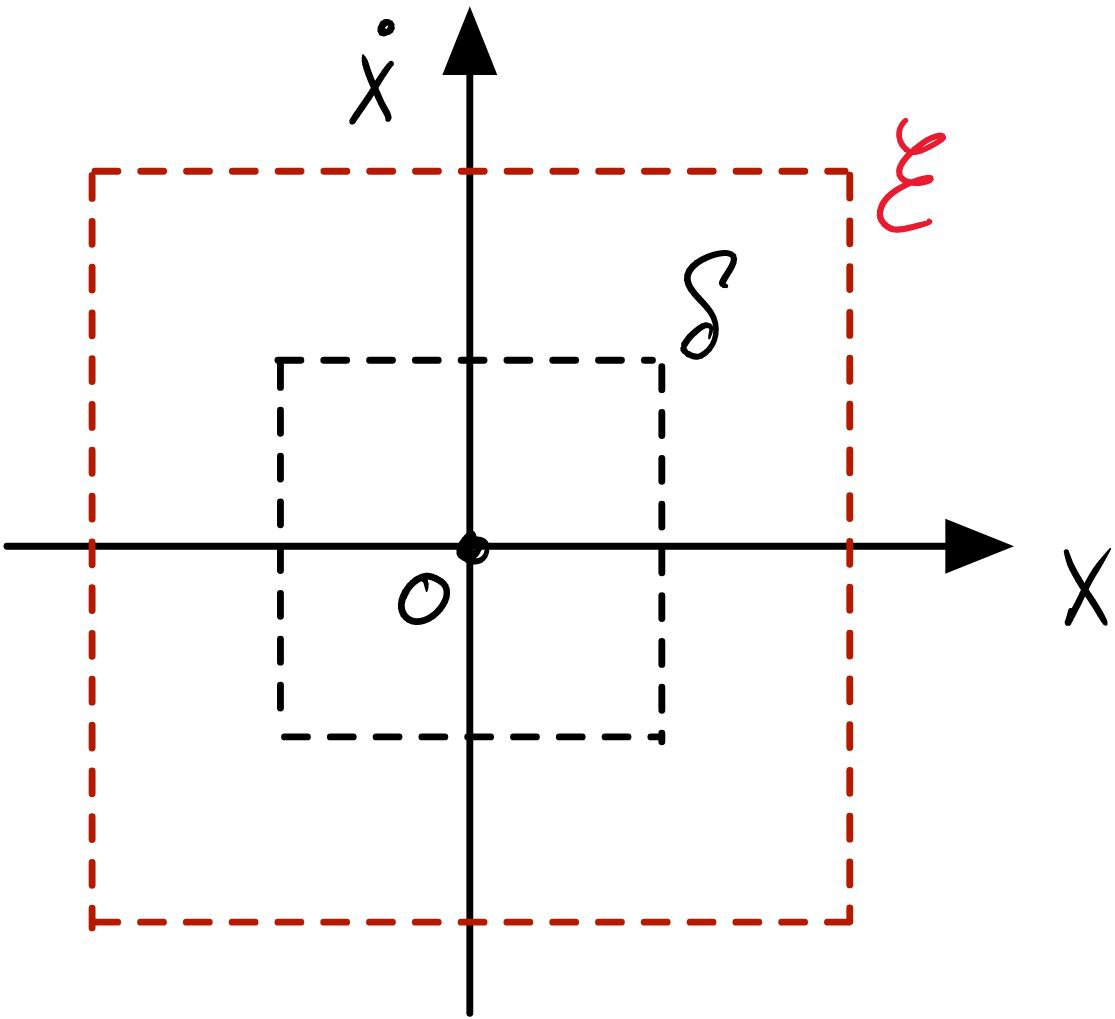
\includegraphics[width=0.8\linewidth]{images/лекция_12_1.jpeg}
\end{wrapfigure}
\tab\\
\begin{definition}
    Точка $x = 0$ --- точка \textbf{устойчивого равновесия}, если $\forall \varepsilon > 0 \exists \delta > 0 : \forall (x(0),~ x'(0)) \in U_\delta(0) \longrightarrow \forall t > 0 (x(t),~\dot{x}(t))\in U_\varepsilon(0)$
\end{definition}

\[
S_3 = \dfrac{(Cr)^2 - 2APa}{2APa}
\]
Рассмотрим два случая.
\begin{enumerate}
    \item \textbf{$S_3 > 1$}\\
    Т.к. $S_3 > 1$, $(Cr)^2 > 4APa$ --- это \textbf{условие Майевского} устойчивости спящего волчка.
    \item \textbf{$S_3 < 1$}\\
    Это неустойчивое движение.
\end{enumerate}
\begin{example}
    Китайский волчок --- \href{https://astrocamp.org/blog/tippe-top/}{tippe top}.
\end{example}
\begin{example}
    Кельтские камни --- \href{https://community.wolfram.com/groups/-/m/t/501324?sortMsg=Likes}{rattleback}.
\end{example}